\chapter{Electromagnetism}

Electromagnetism appears at all length scales.

\section{Electrostatics}

\begin{definition}[Electrostatics]
The physics of \textbf{stationary charges}.
\begin{itemize}
    \item Every particle has an opposite antiparticle with opposite electric charge (e.g.\ electron/positron, proton, antiproton).
    \item Charge is \underline{conserved} and \underline{quantized}.
\end{itemize}
\end{definition}

\subsection{Conservation of Charge}

\begin{theorem}[Conservation of Charge]
If a system is \underline{isolated}, the total charge of that system \underline{does not change}; it is the algebraic sum of $+$ and $-$ charges.
\end{theorem}

\begin{itemize}
    \item Photons can be in/out since they carry no charge.
    \item Charged particles can be created or destroyed but always so as \underline{pairs} (e.g.\ $e^+e^-$ pair production).
\end{itemize}

\subsection{Quantization of Charge}

\begin{definition}[Quantization of Charge]
$e$: smallest discrete unit of charge; in one electron ($e \approx 1.6 \times 10^{-19}$ C).
\begin{itemize}
    \item Protons have exactly the same magnitude of charge: $+e$.
    \item We shall treat charged particles as point particles --- this is a good enough approximation given that the size of charge in a proton is $\sim 10^{-15}$ m, far smaller than relevant scales.
\end{itemize}
\end{definition}

\section{Coulomb's Law}

\begin{formula}[Coulomb's Law]
The force on charge $q_1$ due to charge $q_2$ (where $\hat{r}_{21}$ points from source $q_2$ to test $q_1$):
\[
    \vect{F}_{12} = k \frac{q_1 q_2}{r_{21}^2}\, \hat{r}_{21}, \qquad \text{where } k = \frac{1}{4\pi\varepsilon_0}
\]
By Newton's third law, $\vect{F}_1 = -\vect{F}_2$ (assumes both charges are point particles).
\end{formula}

\subsection{Units and the Constant $k$}

\begin{itemize}
    \item SI unit of charge is the \underline{Coulomb} (C).
    \item Two like charges (each of 1 C) repel with a force of $\approx 8.99 \times 10^9\,\text{N}$ at $1\,\text{m}$ apart.
    \item Thus $k \approx 8.988 \times 10^9\;\dfrac{\text{N}\cdot\text{m}^2}{\text{C}^2}$.
    \item Elementarily, $e \approx 1.602 \times 10^{-19}\,\text{C}$ (1 Coulomb $= 6.242 \times 10^{18}$ electrons).
\end{itemize}

\paragraph{Gaussian System.} In Gaussian units, $k = 1$, so
\[
    \vect{F} = \frac{q_1 q_2}{r^2}\hat{r} \quad\text{(in esu)},
\]
where 1 esu $= \sqrt{\text{dyne}}\cdot\text{cm}$.

\paragraph{SI System.} Alternatively,
\[
    k = \frac{1}{4\pi\varepsilon_0} \implies \varepsilon_0 = \frac{1}{4\pi k} \approx 8.854 \times 10^{-12}\;\frac{\text{C}^2}{\text{N}\cdot\text{m}^2},
\]
so Coulomb's law becomes
\[
    \vect{F} = \frac{1}{4\pi\varepsilon_0}\frac{q_1 q_2}{r_{21}^2}\,\hat{r}_{21}.
\]

\subsection{Significance of Coulomb's Law: Additivity}

Electric charge is \textbf{additive}.
\begin{itemize}
    \item Verifying this requires experimentally measuring charge.
    \item Experiment idea: place charges $q_1$, $q_2$, $q_3$ in series; verify that $q_3 = q_1 + q_2$.
    \item The force with which the charges interact is \emph{not} changed by the presence of a third charge.
\end{itemize}

\begin{theorem}[Superposition Principle]
Combining two sets of sources into one system by placing the second system on top of the first system.
\begin{itemize}
    \item Forces add linearly; the whole is the sum of its parts.
    \item $\displaystyle\vect{F}_a = \sum_{i=1}^{N} \vect{F}_i = \sum_{i=1}^{N} k\frac{q_i q_a}{r_{ia}^2}\,\hat{r}_{ia}$
\end{itemize}
\end{theorem}

\begin{example}[Coulomb's Law: Three Charges]
Place $q_1$ at the origin, $q_2$ at $(d,0)$, $q_3$ at $(0,d)$. The force on $q_1$ from $q_2$ points along $\hat{r}_{12} = -\ihat$:
\[
    \vect{F}_{12} = -\frac{q_1 q_2}{4\pi\varepsilon_0 d^2}\,\ihat.
\]
By superposition, the total force on charge 1:
\[
    \vect{F}_{\text{tot},1} = \vect{F}_{12} + \vect{F}_{13}
    = \frac{q_1 q_2}{4\pi\varepsilon_0 d^2}(-\ihat - \jhat).
\]
\end{example}

\section{Energy in a System of Charges}

\begin{itemize}
    \item Electrical forces are \textbf{conservative}.
    \item How much work does it take to move two charged bodies together from far apart?
\end{itemize}

\begin{formula}[Work to Assemble Two Charges]
\[
    W = \int_{r=\infty}^{r=r_0} \left(-\frac{1}{4\pi\varepsilon_0}\frac{q_1 q_2}{r^2}\right)dr
    = \frac{1}{4\pi\varepsilon_0}\frac{q_1 q_2}{r_0}.
\]
\end{formula}

If you drop a 3rd charge from infinity, the work done by the system becomes:
\begin{align*}
    W_3 &= -\int_{\infty}^{P_3} \vect{F}_{P_3}\cdot d\vect{s} \\
        &= -\int_{\infty}^{P_3} \left(\vect{F}_{q_1} + \vect{F}_{q_2}\right)\cdot d\vect{s} \\
        &= -\int_{\infty}^{P_3} \vect{F}_{q_1}\cdot d\vect{s} - \int_{\infty}^{P_3} \vect{F}_{q_2}\cdot d\vect{s} \\
        &= \frac{q_1 q_3}{4\pi\varepsilon_0 r_{13}} + \frac{q_2 q_3}{4\pi\varepsilon_0 r_{23}}.
\end{align*}

Thus total work in constructing the system is:
\begin{align*}
    W &= W_{12} + W_{13} + W_{23} \\
      &= \frac{1}{4\pi\varepsilon_0}\left(\frac{q_1 q_2}{r_{12}} + \frac{q_1 q_3}{r_{13}} + \frac{q_2 q_3}{r_{23}}\right) \equiv U_e,
\end{align*}
the \emph{energy of the system of charges}.

\begin{formula}[Electric Potential Energy of $N$ Point Charges]
\[
    U = \frac{1}{2}\sum_{i=1}^{N}\sum_{\substack{j=1\\j\neq i}}^{N}
    \frac{1}{4\pi\varepsilon_0}\frac{q_i q_j}{r_{ij}}
    = \frac{1}{8\pi\varepsilon_0}\sum_{i=1}^{N}\sum_{\substack{j=1\\j\neq i}}^{N}
    \frac{q_i q_j}{r_{ij}}.
\]
\end{formula}

\subsection{Electrical Energy in a Crystal Lattice}

\begin{itemize}
    \item On the macroscopic level crystals are nearly neutral.
    \item Goal: calculate the electric potential of an ionic salt/stone.
    \item Notice that in an infinite lattice every ion is in the same position as any other ion of the same type.
    \item Thus $U$ becomes: $U = \frac{1}{2}N\displaystyle\sum_{j \neq 1} \frac{q_1 q_j}{4\pi\varepsilon_0\, r_{1j}}$.
\end{itemize}

Using the central atom as reference (nearest-neighbor distance $a$):
\[
    U = \frac{1}{2}N\frac{e^2}{4\pi\varepsilon_0}\left(-\frac{6e^2}{a} + \frac{12e^2}{\sqrt{2}\,a} + \frac{8e^2}{\sqrt{3}\,a} - \frac{6e^2}{2a} + \cdots\right)
\]
(6 closest, 12 next-closest, 8 furthest-before-that, etc.)
\[
    \approx -\frac{0.874\, Ne^2}{4\pi\varepsilon_0\, a} \quad\text{(negative $\Rightarrow$ formation is energetically favorable)}.
\]

\section{Electric Fields}

\begin{definition}[Electric Field]
Suppose we fix charges $q_1,\ldots,q_N$ in place and want to measure the force on a test charge $q_0$:
\[
    \vect{F} = \sum_{i=1}^{N} k\frac{q_i q_0}{r_{i0}^2}\hat{r}_{i0}
    = q_0\,\vect{E} \quad \Longrightarrow \quad \vect{E} \text{ is the \textbf{Electric Field}.}
\]
The electric field provides a \emph{local} property which allows us to not have to take into account the change of $q_0$ to predict the function of the electric field.
\end{definition}

\subsection{Visualizing Electric Fields}

\begin{itemize}
    \item \textbf{Field lines:} Curves whose tangent at any point lies in the direction of the field at that point.
    \item Density of field lines represents magnitude.
\end{itemize}

\begin{figure}[H]
\begin{center}
\begin{tikzpicture}[scale=1.1]
  % Radial field lines from a positive point charge
  \foreach \angle in {0,30,60,90,120,150,180,210,240,270,300,330} {
    \draw[-{Stealth[length=5pt]}, thick, blue!70!black]
      (0,0) -- ({1.5*cos(\angle)},{1.5*sin(\angle)});
  }
  % Charge
  \filldraw[red] (0,0) circle (4pt) node[below right, black]{$+q$};
  % Label
  \node at (0,-2.0) {Electric field lines radiating from $+q$};
\end{tikzpicture}
\end{center}
\caption{Field lines radiating outward from a positive point charge $+q$. The density of lines represents the field magnitude, which falls as $1/r^2$.}
\end{figure}

\subsection{Electric Force on a Test Charge}

\[
    \vect{F} = q\vect{E} \quad \text{(force on a test charge $q$)}.
\]

\section{Continuous Charge Distributions}

\begin{definition}[Charge Density]
$\rho = f(x,y,z)$ has units of charge/volume or charge/area.
\[
    \rho\,dV = dQ, \quad dV = dx\,dy\,dz.
\]
\end{definition}

\begin{formula}[Electric Field from a Continuous Distribution]
\[
    \vect{E}(x,y,z) = \frac{1}{4\pi\varepsilon_0}
    \int \frac{\rho(x',y',z')\,\hat{r}\,dV'}{r^2}
    \quad \text{(volume integral)},
\]
where $\hat{r}$ points \emph{from source} $(x',y',z')$ \emph{to test point} $(x,y,z)$ (i.e.\ from source to test charge; $\hat{r}$ is always this direction).
\end{formula}

\subsection{Example: Field Due to a Hemisphere (Finite)}

\begin{example}[Hemisphere]
Consider a uniformly charged hemisphere with surface charge density $\sigma$.

Using spherical coordinates, the area element is $d\sigma = r^2\sin\theta\,d\theta\,d\phi$, so $dV = r^2\sin\theta\,dr\,d\theta\,d\phi$. Setting $dQ = \rho\,dV$, by symmetry the horizontal components of $\vect{E}$ cancel due to rotational symmetry, giving:
\[
    dE_z = \frac{\rho(2\pi r^2 \sin\theta\,dr\,d\theta)\cos\theta}{4\pi\varepsilon_0\, r^2}.
\]
\[
    E_z = \int_0^{\pi/2}\int \frac{\rho\cdot 2\pi r^2 \sin\theta\cos\theta}{4\pi\varepsilon_0\, r^2}\,dr\,d\theta
        = \frac{\rho}{2\varepsilon_0}\cdot R\cdot \frac{\sin^2\theta}{2}\Bigg|_0^{\pi/2}
        = \frac{\rho R}{4\varepsilon_0}.
\]

\textbf{Note:} Because the volume of a ring grows as $r^2$, this cancels the $\frac{1}{r^2}$ denominator, which removes the singularity.
\end{example}

\subsection{Example: Field on a Ring}

\begin{example}[Uniform Ring]
A ring of charge $Q$ and radius $R$. Find the field at a point $P$ on the axis at distance $x$ from the center.

\[
    |d\vect{E}| = \frac{dQ}{4\pi\varepsilon_0}\cdot\frac{1}{R^2 + x^2}.
\]

The $x$-component (along the axis):
\[
    dE_x = \frac{1}{4\pi\varepsilon_0}\frac{x\,dQ}{(R^2+x^2)^{3/2}}.
\]
By symmetry, the transverse components cancel. What about $z$? They cancel by symmetry too.

Integrating over the full ring ($\int dQ = Q$):
\[
    E_x = \frac{1}{4\pi\varepsilon_0}\frac{x\,Q}{(R^2+x^2)^{3/2}}.
\]
\end{example}

\subsection{Example: Uniform Disk}

\begin{example}[Uniform Disk]
Surface charge density $\sigma = Q/(\pi R^2)$.

Build the disk from rings of radius $r$ and width $dr$: $dQ = \sigma \cdot 2\pi r\,dr$.

Using the ring result:
\[
    \vect{E} = E_x\,\ihat = \frac{\sigma x}{2\varepsilon_0}
    \int_0^R \frac{r\,dr}{(r^2+x^2)^{3/2}}\,\ihat.
\]

Evaluate the integral:
\[
    E_x = \frac{\sigma}{2\varepsilon_0}\left(1 - \frac{1}{\sqrt{1+R^2/x^2}}\right).
\]

\paragraph{Infinite plane limit ($R\to\infty$):}
\[
    E_x \to \frac{\sigma}{2\varepsilon_0}.
\]

\paragraph{Far-field limit ($x \gg R$, finite disk):}
Using $(1+a)^n \approx 1 + na$ for small $a$:
\begin{align*}
    \sqrt{1+R^2/x^2} &\approx 1 + \frac{1}{2}\frac{R^2}{x^2}, \\
    E_x &\approx \frac{\sigma}{2\varepsilon_0}\left(1 - \frac{1}{1 + \frac{R^2}{2x^2}}\right)
          \approx \frac{\sigma}{2\varepsilon_0}\cdot\frac{R^2}{2x^2}
          = \frac{\sigma \pi R^2}{4\pi\varepsilon_0 x^2}
          = \frac{Q}{4\pi\varepsilon_0 x^2}.
\end{align*}
As expected, the finite disk looks like a point charge from far away.
\end{example}

\section{Flux and Gauss's Law}

\subsection{Flux}

\begin{definition}[Electric Flux]
Approximate a smooth, closed 3D shape by a bunch of flat rectangles with normals $\hat{n}$. Let $\vect{E}$ be the electric field at $d\vect{A}$. The flux through a surface element is $\vect{E}\cdot d\vect{A}$.

Generalizing, the flux through a surface $S$ is:
\[
    \Phi = \int_S \vect{E}\cdot d\vect{A} = \int_S \partial A\,(\hat{n}\cdot\vect{E}).
\]
\end{definition}

\begin{itemize}
    \item Flux represents the magnitude.
    \item For a closed surface: $\displaystyle\oint_S \vect{E}\cdot d\vect{A} = \frac{Q_\text{enc}}{\varepsilon_0}$.
\end{itemize}

\subsection{Derivation of Gauss's Law from Coulomb's Law}

Consider a simple system consisting of a single point charge (source) $q$ and use a hollow sphere of radius $r$ as the Gaussian surface.

\begin{figure}[H]
\begin{center}
\begin{tikzpicture}[scale=1.0]
  % Gaussian sphere
  \draw[dashed, thick, blue!60!black] (0,0) circle (1.6);
  \node[blue!60!black] at (1.8,1.2) {Gaussian surface};
  % charge at center
  \filldraw[red] (0,0) circle (4pt) node[below right, black]{$+q$};
  % field lines through sphere
  \foreach \angle in {0,45,90,135,180,225,270,315} {
    \draw[-{Stealth[length=5pt]}, thick, orange!80!black]
      ({0.5*cos(\angle)},{0.5*sin(\angle)}) -- ({1.6*cos(\angle)},{1.6*sin(\angle)});
  }
  % normal vector arrow
  \draw[-{Stealth[length=6pt]}, thick, green!60!black]
    ({1.6*cos(45)},{1.6*sin(45)}) -- ({2.2*cos(45)},{2.2*sin(45)})
    node[above right, black]{$d\vect{A} = \hat{r}\,dA$};
  % radius label
  \draw[thin, gray] (0,0) -- ({1.6*cos(200)},{1.6*sin(200)}) node[midway, right]{$r$};
\end{tikzpicture}
\end{center}
\caption{Gaussian surface (dashed sphere of radius $r$) enclosing point charge $+q$. At every point the field $\vect{E}$ is radial and constant in magnitude, so $\Phi = E \cdot 4\pi r^2 = q/\varepsilon_0$.}
\end{figure}

At every point on the sphere, $\vect{E} = \dfrac{q}{4\pi\varepsilon_0 r^2}\,\hat{r}$. Then:
\[
    \Phi = \oint \vect{E}\cdot d\vect{A} = E\cdot(4\pi r^2) = \frac{q}{4\pi\varepsilon_0 r^2}\cdot 4\pi r^2 = \frac{q}{\varepsilon_0}.
\]
(This only works because $E$ is constant on the surface.)

\paragraph{Surprising fact:} The net flux through \emph{any} surface that encloses the point charge is the same $q/\varepsilon_0$.

\begin{figure}[H]
\centering
\caption{An irregular closed surface enclosing a point charge $q$. A cone of solid angle element intersects both the irregular surface and a concentric sphere. By similar triangles, the areas scale as $L^2/R^2$, so $A = (L/R)^2\,a\cos\theta$, giving the same flux on both surfaces: $E_r\,a$.}
\end{figure}

Thus the flux through the outer patch equals the flux on the inner patch: $E_r\,a$.

\textbf{Corollary:} The total flux through a closed surface is \emph{zero} if the point charge lies \emph{outside} the surface.

Superposition principle holds for flux:
\[
    \Phi = \int_S \vect{E}\cdot d\vect{A}
         = \int_S (\vect{E}_1 + \vect{E}_2 + \cdots + \vect{E}_N)\,d\vect{A}.
\]

\begin{fact}[Gauss's Law]
\[
    \oint \vect{E}\cdot d\vect{A} = \frac{Q_\text{enc}}{\varepsilon_0}
    = \frac{1}{\varepsilon_0}\sum_i q_i
    = \frac{1}{\varepsilon_0}\int \rho\,dV.
\]
\begin{itemize}
    \item Coulomb's Law: charges $\to$ electric field.
    \item Gauss's Law: electric field $\to$ charges.
\end{itemize}
\end{fact}

\subsection{Applying Gauss's Law: Only 3 Useful Cases}

The catch: Gauss's Law is only $\Phi = E\cdot A$ when $|\vect{E}|$ is constant on the surface.

\begin{itemize}
    \item Case (1): Sphere with $\sigma = \text{const}$ (field inside is $\vect{E} = 0$, field is only radially outward). Works.
    \item Case (2): A box (cube) $\Rightarrow$ $\vect{E}$ is only \emph{average} zero; it is not zero at every point. Does \emph{not} work in general.
\end{itemize}

Only three cases where Gauss's Law can be applied to extract $E$ simply:
\begin{enumerate}
    \item \textbf{Spherical charge:} $|\vect{E}_\text{sphere}| = \dfrac{Q}{4\pi\varepsilon_0 r^2}$.
    \item \textbf{Infinite line charge:} $|\vect{E}| = \dfrac{\lambda}{2\pi\varepsilon_0 r}$.
    \item \textbf{Infinite sheet:} $|\vect{E}_\text{sheet}| = \dfrac{\sigma}{2\varepsilon_0}$.
\end{enumerate}

\subsection{Example: Gauss's Law on a Spherical Surface}

\begin{example}[Point Charge Inside a Hollow Sphere]
Find the charge on a point inside a hollow sphere with $\rho = Q/(\frac{4}{3}\pi R^3)$.

By Gauss's Law, for a Gaussian sphere of radius $r_1$:
\[
    E_r \cdot 4\pi r_1^2 = \frac{Q_\text{enc}}{\varepsilon_0}
    \implies E_r = \frac{Q_\text{enc}}{4\pi\varepsilon_0\, r_1^2}.
\]
For $r_1 < r_2$, using $E_r\cdot 4\pi r^2 = Q(r^3/R^3)/\varepsilon_0$:
\[
    E_r = \frac{Q\, r}{4\pi\varepsilon_0\, R^3}.
\]
\end{example}

\subsection{Example: Gauss's Law on a Spherical Charge Distribution}

\begin{example}[Uniform Spherical Charge Distribution]
For a sphere of uniform charge density $\rho$, total charge $Q$:

\[
    \Phi = E_r\cdot 4\pi r_1^2 = \frac{Q_\text{enc}}{\varepsilon_0}
    \implies E_r = \frac{Q_\text{enc}}{4\pi\varepsilon_0\, r_1^2}.
\]
The field at any point on $S_2$ is the same as if all charge within $S_2$ were at the center.

If $r_1 \geq r_2$ (outside), with density now constant:
\[
    E(r) = \frac{\frac{4}{3}\pi r^3\,\rho}{4\pi\varepsilon_0\,r^2} = \frac{\rho\, r}{3\varepsilon_0}.
\]

For $r \leq R$, the charge outside $R$ contributes nothing while the charge inside always acts as if it is at the center:
\[
    E(r) = \frac{\frac{4}{3}\pi r^3\,\rho}{4\pi\varepsilon_0\,r^2} = \frac{\rho\, r}{3\varepsilon_0}.
\]

\begin{figure}[H]
\begin{center}
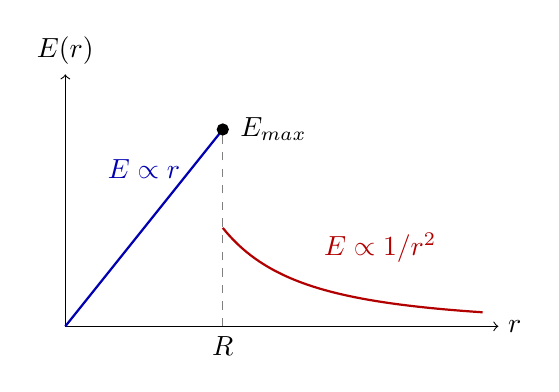
\begin{tikzpicture}[scale=1.0]
  \draw[->] (0,0) -- (5.5,0) node[right]{$r$};
  \draw[->] (0,0) -- (0,3.2) node[above]{$E(r)$};
  % sphere radius marker
  \draw[dashed, gray] (2,0) -- (2,2.5);
  \node[below] at (2,0) {$R$};
  % inside: linear rise from 0 to E_max at R
  \draw[thick, blue!70!black, domain=0:2, samples=40]
    plot (\x, {1.25*\x});
  % outside: 1/r^2 fall from R outward
  \draw[thick, red!70!black, domain=2:5.3, samples=80]
    plot (\x, {5.0/(\x*\x)});
  % peak marker
  \filldraw[black] (2,2.5) circle (2pt);
  \node[right] at (2.1,2.5) {$E_\text{max}$};
  % labels
  \node[blue!70!black] at (1.0,2.0) {$E \propto r$};
  \node[red!70!black] at (4.0,1.0) {$E \propto 1/r^2$};
\end{tikzpicture}
\end{center}
\caption{Electric field magnitude vs.\ radius for a uniformly charged sphere of radius $R$: rises linearly inside ($E \propto r$), peaks at $r=R$, and falls as $1/r^2$ outside.}
\end{figure}
\end{example}

\subsection{Electric Field on a Line Charge}

\begin{example}[Infinite Line Charge]
$\lambda$ = linear charge density (coulombs/meter).

\textbf{Traditional method:} By symmetry $\vect{E}$ must point in the $\hat{y}$ direction.
\[
    dq = \lambda\,dx, \quad dE_y = \frac{dq}{4\pi\varepsilon_0\, R^2}\cos\theta.
\]
\[
    E_y = \int_{-\infty}^{\infty} \frac{\lambda\cos\theta\,dx}{4\pi\varepsilon_0\, R^2}.
\]
Using $R = r/\cos\theta$ and $dx = r\,d\theta/\cos^2\theta$, thus:
\[
    E_y = \int_{-\pi/2}^{\pi/2} \frac{\lambda\cos\theta}{4\pi\varepsilon_0\, r}\,d\theta
        = \frac{\lambda}{4\pi\varepsilon_0\, r}\cdot 2
        = \frac{\lambda}{2\pi\varepsilon_0\, r}.
\]

\textbf{Using Gauss's Law:} Flux through the cylindrical surface is $2\pi r L \cdot E_r$; by Gauss's Law $= \lambda L/\varepsilon_0$:
\[
    E_r = \frac{\lambda}{2\pi\varepsilon_0\, r}.
\]

\begin{figure}[H]
\begin{center}
\begin{tikzpicture}[scale=0.9]
  % Line charge (vertical dashed line)
  \draw[dashed, thick, red!70!black] (0,-2.2) -- (0,2.2) node[above]{$\lambda$};
  % Gaussian cylinder (drawn as ellipse + rectangle)
  \draw[blue!70!black, thick] (0,1.2) ellipse (1.5 and 0.35);
  \draw[blue!70!black, thick] (0,-1.2) ellipse (1.5 and 0.35);
  \draw[blue!70!black, thick] (-1.5,-1.2) -- (-1.5,1.2);
  \draw[blue!70!black, thick] (1.5,-1.2) -- (1.5,1.2);
  % Radius label
  \draw[<->, gray] (0,0) -- (1.5,0) node[midway, above]{$r$};
  % Length label
  \draw[<->, gray] (1.8,-1.2) -- (1.8,1.2) node[midway, right]{$L$};
  % Outward field arrows on cylinder side
  \draw[-{Stealth[length=5pt]}, thick, orange!80!black] (1.5,0.5) -- (2.3,0.5) node[right]{$\vect{E}$};
  \draw[-{Stealth[length=5pt]}, thick, orange!80!black] (-1.5,0.5) -- (-2.3,0.5);
  \draw[-{Stealth[length=5pt]}, thick, orange!80!black] (1.5,-0.5) -- (2.3,-0.5);
  \draw[-{Stealth[length=5pt]}, thick, orange!80!black] (-1.5,-0.5) -- (-2.3,-0.5);
  % End cap: no flux label
  \node[blue!60!black, font=\small] at (2.5,-1.8) {Gaussian cylinder};
\end{tikzpicture}
\end{center}
\caption{Gaussian cylindrical surface of radius $r$ and length $L$ coaxial with an infinite line charge $\lambda$. The field is purely radial on the curved surface; end caps contribute no flux.}
\end{figure}
\end{example}

\subsection{Electric Field of an Infinite Flat Sheet of Charge}

\begin{example}[Infinite Plane Sheet]
By symmetry $\vect{E}$ must point away from (or toward) the plane.

Choose a Gaussian cylinder of cross-section $A$ straddling the sheet:
\[
    AE_\text{top} + AE_\text{bot} = 2AE_P = \frac{\sigma A}{\varepsilon_0}
    \implies \boxed{E_P = \frac{\sigma}{2\varepsilon_0}}.
\]
The Gaussian surface must have flux in the same direction as the given shape, and must have the same flux at all relevant points.

\begin{figure}[H]
\begin{center}
\begin{tikzpicture}[scale=0.95]
  % Infinite sheet
  \fill[orange!20] (-3,-0.12) rectangle (3,0.12);
  \draw[thick, orange!70!black] (-3,0) -- (3,0) node[right]{$\sigma$};
  % Gaussian pillbox (cylinder straddling sheet)
  \draw[blue!70!black, thick] (0,0.9) ellipse (1.1 and 0.27);
  \draw[blue!70!black, thick] (0,-0.9) ellipse (1.1 and 0.27);
  \draw[blue!70!black, thick] (-1.1,-0.9) -- (-1.1,0.9);
  \draw[blue!70!black, thick] (1.1,-0.9) -- (1.1,0.9);
  % Area label
  \node[blue!60!black] at (0.4,0.6) {$A$};
  % Upward field arrow (top cap)
  \draw[-{Stealth[length=6pt]}, thick, red!70!black] (0,0.9) -- (0,1.7) node[above]{$\vect{E}$};
  % Downward field arrow (bottom cap)
  \draw[-{Stealth[length=6pt]}, thick, red!70!black] (0,-0.9) -- (0,-1.7) node[below]{$\vect{E}$};
  % Side walls: no flux
  \node[font=\small, gray] at (1.9,0) {(no flux on side)};
  \node[blue!60!black, font=\small] at (-2.5,-1.3) {Gaussian pillbox};
\end{tikzpicture}
\end{center}
\caption{Gaussian pillbox straddling an infinite sheet with surface charge density $\sigma$. The field exits symmetrically through both end caps of area $A$; no flux through the side walls.}
\end{figure}
\end{example}

\section{Force on a Layer of Charge}

\begin{itemize}
    \item Surface charge density $\sigma$, inside a hollow sphere.
    \item Inside the sphere the electric field is 0.
    \item Outside the sphere the field is $\dfrac{Q}{4\pi\varepsilon_0 r^2}$.
    \item So just outside the sphere, when $r = r_0$: $E_\text{outside} = \dfrac{\sigma}{\varepsilon_0}$ by Gauss's Law.
\end{itemize}

\textbf{Q: What is the electrical force experienced by the charges that make up this distribution?}

Force of a patch on itself: 0 (by Newton's third law). Total forces on the patch:
\[
    d\vect{F} = E\,q_\text{patch} = E\,\sigma\,dA.
\]
\[
    d\vect{F} = \frac{1}{2}(E_\text{inside} + E_\text{outside})\,\sigma\,dA
              = \frac{1}{2}\left(\frac{\sigma}{\varepsilon_0}\right)\sigma\,dA
    \implies d\vect{F} = \frac{\sigma^2}{2\varepsilon_0}\,dA.
\]

More generally, consider a Gaussian surface where the field changes continuously from $E_1$ to $E_2$. Gauss's Law says $E_2 - E_1 = \sigma/\varepsilon_0$ for Gaussian surfaces:
\begin{align*}
    \frac{F}{A} &= \int_0^{x_0} E(x)\,\rho(x)\,dx \\
    \frac{E}{A} &= \int_{x_0}^{x_0} E_0\,\varepsilon_0\,dE = \varepsilon_0\left(\frac{E_2^2 - E_1^2}{2}\right)
                 = \varepsilon_0(E_2 - E_1)\frac{E_2+E_1}{2}.
\end{align*}
\begin{formula}[Force per Unit Area on a Charge Layer]
\[
    \frac{F}{A} = \frac{1}{2}(E_1 + E_2)\,\sigma\,\frac{\sigma}{\varepsilon_0}
    \quad \Longrightarrow \quad
    \frac{F}{A} = \frac{1}{2}(E_\text{inside} + E_\text{outside})\,\sigma.
\]
\end{formula}

The direction of the electrical force is \emph{outward} no matter whether the surface charge is positive or negative.

\section{Energy Density of the Electric Field}

Take a hollow shell: $E_\text{inside} = 0$, $E_\text{outside} = \dfrac{\sigma\cdot 4\pi r^2}{4\pi\varepsilon_0} = \dfrac{Q}{4\pi\varepsilon_0 r^2}$.

\[
    \lim_{r\to r^+} E_\text{just outside} = \frac{\sigma}{\varepsilon_0}
    \quad \left(\text{why not } \frac{\sigma}{2\varepsilon_0}?\right)
\]

\paragraph{Squeezing the sphere:} The field inside is 0, outside is $\sigma/\varepsilon_0$; average is $\sigma/(2\varepsilon_0)$. So avg.\ $E = \dfrac{\sigma}{2\varepsilon_0}$.

Work done in squeezing the shell inward by $dr$:
\begin{align*}
    dW &= \frac{\sigma^2}{2\varepsilon_0}\cdot 4\pi r^2\,dr \\
    dW &= \frac{1}{2}\varepsilon_0 E^2\,dV.
\end{align*}

\begin{formula}[Energy Density of the Electric Field]
\[
    u_E = \frac{1}{2}\varepsilon_0 E^2 \quad \text{(energy density)}.
\]
\end{formula}


\subsection{Example: Potential Energy of a Uniform Sphere}

\begin{example}[PE of a Uniform Sphere]
Outside the sphere, the field at radius $r$ is $Q/(4\pi\varepsilon_0 r^2)$, so the energy stored is:
\[
    U_\text{ext} = \frac{\varepsilon_0}{2}\int_R^{\infty}\left(\frac{Q}{4\pi\varepsilon_0 r^2}\right)^2 4\pi r^2\,dr
                 = \frac{Q^2}{8\pi\varepsilon_0 R}.
\]

We know from before that $E_r = \dfrac{\rho r}{3\varepsilon_0}$ inside. But the density is $\rho = Q/\!\left(\frac{4}{3}\pi R^3\right)$; thus:
\[
    E_r = \frac{3\rho}{4\pi\varepsilon_0}\cdot\frac{r}{R^3} = \frac{Qr}{4\pi\varepsilon_0 R^3}.
\]

Thus:
\begin{align*}
    U_\text{int} &= \frac{\varepsilon_0}{2}\int_0^R \left(\frac{Qr}{4\pi\varepsilon_0 R^3}\right)^2 4\pi r^2\,dr \\
                 &= \frac{Q^2}{8\pi\varepsilon_0 R^6}\int_0^R r^4\,dr
                  = \frac{Q^2}{8\pi\varepsilon_0}\cdot\frac{1}{5R}.
\end{align*}

\[
    U_\text{tot} = U_\text{int} + U_\text{ext} = \frac{5Q^2}{8\cdot 5\pi\varepsilon_0 R}
                 = \frac{3Q^2}{20\pi\varepsilon_0 R}.
\]

\noindent (The inner integral over $r = 0$ to $r = R$: $\displaystyle\int_0^R \frac{Qr^3}{R^3}\cdot\frac{Q}{4\pi r^2}\,4\pi r^2\,dr$, evaluated at $r = R$.)
\end{example}

\section{Chapter Summary}

\subsection{Forces Between Two Charges}
\[
    \vect{F} = \frac{1}{4\pi\varepsilon_0}\frac{q_1 q_2}{r_{21}^2}\,\hat{r}_{21}.
\]

\subsection{Potential Energy of a System of Charges}
\[
    U = \frac{1}{2}\sum_{j=1}^{N}\sum_{\substack{k=1\\k\neq j}}^{N}
    \frac{1}{4\pi\varepsilon_0}\frac{q_j q_k}{r_{jk}}.
\]

\subsection{Electric Field Due to a Charge Distribution}
\[
    \vect{E} = \frac{1}{4\pi\varepsilon_0}\int \frac{\rho(x',y',z')\,\hat{r}\,dx'\,dy'\,dz'}{r^2}
    \quad \text{or} \quad
    \frac{1}{4\pi\varepsilon_0}\sum_{j=1}^{N}\frac{q_j\,\hat{r}_j}{r_j^2}.
\]
\[
    \vect{F} = q\vect{E} \quad \text{(force on a test charge)}.
\]

\subsection{Flux of an Electric Field through Surface $S$}
\[
    \Phi = \int_S \vect{E}\cdot d\vect{A}.
\]

\begin{fact}[Gauss's Law (Summary)]
Flux of an $\vect{E}$ through any closed surface:
\[
    \oint \vect{E}\cdot d\vect{A} = \frac{1}{\varepsilon_0}\int \rho\,dV = \frac{1}{\varepsilon_0}\sum q_i = \frac{Q_\text{enc}}{\varepsilon_0}.
\]
Pre-determined shapes:
\[
    E_\text{sphere} = \frac{Q}{4\pi\varepsilon_0 r^2}, \quad
    E_\text{line} = \frac{\lambda}{2\pi\varepsilon_0 r}, \quad
    E_\text{sheet} = \frac{\sigma}{2\varepsilon_0}.
\]
\end{fact}

\begin{itemize}
    \item Force per unit area on a layer of charge:
    \[
        \frac{F}{A} = \frac{1}{2}(E_\text{inside} + E_\text{outside})\,\sigma.
    \]
    \item Energy density of an electric field is $\dfrac{\varepsilon_0 E^2}{2}$, so:
    \[
        U = \frac{\varepsilon_0}{2}\int E^2\,dV \quad\Longrightarrow\quad
        \text{represents the total work required to assemble a system of charges.}
    \]
\end{itemize}

\subsection{Handy Trig Substitutions}

For integrals of the form $\dfrac{1}{(x^2+a^2)^n}$, use $x = a\tan(u)$:
\[
    \implies dx = a\sec^2(u)\,du.
\]

\section{Selected Problems}

\subsection{Problem 1.13 --- Hole in a Plane}

\begin{example}[Hole in a Plane]
An infinite plane with a hole of radius $R$. Find the field at a point $z$ above the hole.

\textbf{Strategy:} Find the field due to the entire plane, then subtract the field from the disk of radius $R$.

By Gauss's Law for the entire plane:
\[
    2(\vect{E}\cdot\pi R^2) = \frac{\sigma\pi R^2}{\varepsilon_0}
    \implies \vect{E} = \frac{\sigma}{2\varepsilon_0}.
\]

Minus the disk: $dq = \sigma\cdot 2\pi r\,dr$.
\[
    \text{thus } dE = \frac{1}{4\pi\varepsilon_0}\frac{2\pi r\,\sigma\,dr\,z}{(z^2+r^2)^{3/2}}.
\]
\[
    E_\text{disk} = \frac{\sigma z}{2\varepsilon_0}\int_0^R\frac{r\,dr}{(z^2+r^2)^{3/2}}
                  = \frac{\sigma z}{2\varepsilon_0}\cdot\frac{-1}{(z^2+r^2)^{1/2}}\Bigg|_0^R
                  = \frac{\sigma z}{2\varepsilon_0}\left(\frac{-1}{(R^2+z^2)^{1/2}} + \frac{1}{z}\right).
\]
\[
    \text{Thus} \quad \boxed{E_\text{hole} = \frac{\sigma z}{2\varepsilon_0(z^2+R^2)^{1/2}}}.
\]
\end{example}

